\documentclass[a4paper, 12pt]{article}

\usepackage{float}
\usepackage{amsmath, amsthm, amssymb}
\usepackage{graphicx}
\usepackage{enumitem}
\usepackage{booktabs}
\usepackage{url}
\usepackage{float}
\usepackage{caption}
\usepackage{subcaption}

\numberwithin{equation}{section}
\setlength{\parindent}{0pt}
\setlist[itemize]{itemsep=1pt, topsep=1pt}

\begin{document}
	
	\title{Study of Gentrification \\ in the New York Metropolitan Area}
	\author{Citadel European Regional Datathon \\
		\\
		Dmitry Silantyev \\
		Padmanaba Srinivasan \\
		Stefan Tionanda \\
		Bahdan Zviazhynski \\
	} 
	\date{\today}
	\maketitle
	
	\pagenumbering{roman}
	\tableofcontents
	\newpage
	\pagenumbering{arabic}
	
	\section{Executive Summary}
			
		In this report, we set out to develop a robust methodology to identify areas with ongoing gentrification. Despite ample anecdotal evidence, there is still no unifying framework that allows to pin down specific census tracts as subject to gentrification, let alone make conclusion about cause and effect of the phenomenon. Perhaps the starkest illustration of this is a recent study by Preis et al. \cite{Preis20} that applied four different methodologies to the Boston area and found only seven tracts identified as gentrifying or at risk by all four methods. Having reproduced the often-cited algorithm of Prof. Freeman from Columbia University \cite{Freeman05} (henceforth referred to as the Columbia or the Governing Magazine method) and compared it to the results of a group of researchers from UC Berkeley \cite{Chapple17}, we also found the number of overlapping tracts to be in low double digits. This result has often been attributed by researchers to the difference in city-specific assumptions about what gentrification is. Here, we propose a simple and elegant clustering algorithm that is theory-agnostic yet powerful in identifying areas that have meaningfully different statistical properties comparing to their population and that can serve as an aid in policy making. \\
		
		While the picture painted in the BuzzFeed article and the Governing report is that of newcomers (mostly white and better educated) displacing inhabitants of historically non-white neighbourhoods by pricing them out, averages taken across the metropolitan area don't yet lend support to this story. Over the course of 2009-18, the share of population with at least a bachelor's degree grew by only 2 p.p. and the share of Hispanic population (+3 p.p.) increased at the expense of white (-5 p.p.) and African American (-1 p.p.) groups (see Table \ref{tab:dist}). Correlations (see Figure \ref{fig:corr}), while being in line with the story, are modest in magnitude and don't indicate existence of strong linear relationships between variables (except in the case of race-based variables that are tied by linear relationship by definition and the link between higher educational attainment and income, which is not related to gentrification per se). Even more surprisingly, tracts identified as gentrifying based on the methodology designed by Governing \cite{Governing15} (relying on trends in education, income and home prices), do not reveal almost any pattern in the corresponding racial dynamic or crime data that we collected separately (see Figure \ref{fig:distr_gov}). \\
		
			\begin{figure}[H]
				\centering
				\includegraphics[width=0.75\linewidth]{figs/"corr_changes.png"}
				\caption{Correlation Matrix for Changes over 2009-18}
				\label{fig:corr}
			\end{figure}
		
		Since there is no consensus about which properties a gentrifying tract should exhibit, this problem cannot be cast into a supervised classification problem for a machine learning algorithm. Therefore, without imposing any specific set of assumptions, we ran a series of unsupervised clustering algorithms to see if they can pick up some structure in the data. The results are very promising, as one can see in Figure \ref{fig:distr}. Out of $\approx$4,000 census tracts in New York metropolitan area, our best iteration of K-Means Clustering algorithm found a cluster of 130 tracts that all exhibit the pattern described by BuzzFeed, i.e. an ongoing displacement of African American and Hispanic populations by educated white newcomers, associated with a rapid increase in median income and median house price. Statistical tests conducted to see if the distribution of changes in the analysed variables across all tracts is different from that for the cluster, all confirm that the distributions are distinct in statistical sense. In that group, which we will further refer to as gentrified tracts, average (across tracts) median (within tract) income increased by 86\% in 2009-18, the share of population with at least a bachelor's degree increased by 10 p.p. and an increase in the share of white population (+10 p.p.) was associated with a material decrease in non-white population (-6 p.p for African American and - 7 p.p. for Hispanic).
		
		\begin{figure}[H]
			\centering
			\includegraphics[width=1\linewidth]{figs/"kmeans_cluster_gentr.png"}
			\caption{Distribution of Changes in All Tracts vs. Gentrified Tracts}
			\label{fig:distr}
		\end{figure}
	
		\begin{table}[H]
			\centering
			\resizebox{\textwidth}{!}{
			\begin{tabular}{|l|c|c|c|c|c|}
			 \multicolumn{2}{c}{} &  \multicolumn{2}{c}{Mean}  &  \multicolumn{2}{c}{St. Dev.} \\ \hline
			 &  KS p-val &  All  &  Gent. &  All  &  Gent. \\ \hline 
			$\Delta$ Median Income, \%  & 0.0 *** & 21.904 & 85.560 & 26.781 & 39.267 \\ \hline
			$\Delta$ Educ. Attainment, pp &  0.0 *** & 2.018 & 10.520 & 4.391 & 5.301 \\ \hline
			$\Delta$ Median Home Value, \%  & 0.0 *** & 8.046 & 54.250 & 47.301 & 60.731 \\ \hline 
			$\Delta$ White Population, pp & 0.0 *** & -4.923 & 9.920 & 8.711 & 8.413 \\ \hline 
			$\Delta$ Black Population, pp & 0.0 *** & -0.792 & -5.983 & 6.344 & 9.513 \\ \hline 
			$\Delta$ Hispanic Population, pp & 0.0 *** & 2.996 & -7.294 & 7.656 & 8.833 \\ \hline 
			\end{tabular}}
				\caption{Kolmogorov-Smirnov Test Results and Distribution Statistics}
				\label{tab:dist}
		\end{table}
		
		Out of 130 tracts identified as distinct by K-Means Clustering and interpreted as gentrifying by us, only 14 overlap with tracts picked by our implementation of the Governing methodology. However, 106 tracts in the cluster are classified by the group of researchers from UC Berkeley as undergoing some form of exclusion or gentrification, ranging from "Ongoing Exclusion" to "Advanced Gentrification". \\
		
		In order to ensure the validity of our findings out-of-sample, we reserve several variables as external, following a similar approach taken by Freeman \cite{Freeman05}. One of reserved variables is the percentage change in the number of violent crimes committed on the territory of a tract and sourced from Crime Open Data Base (CODE) for over 1,000 census tracts in New York City. Here the difference between gentrified and non-gentrified tracts is not so stark but still supports our thesis: while the number of violent crimes declined by 4.6\% in NYC over 2009-18, it fell by 8.5\% in gentrified tracts. Figure \ref{fig:crime} illustrates this point as more tracts identified by our algorithm as gentrifying saw a material decrease in violent crime rates, comparing to the all tracts in New York City for which crime data was available.

		\begin{figure}[H]
			\centering
			\includegraphics[width=0.75\linewidth]{figs/"all_vs_gent_change_in_crime.png"}
			\caption{Distribution of \% Changes in Number of Violent Crimes  in All Tracts vs. Gentrified Tracts}
			\label{fig:crime}
		\end{figure}
		
	    The other way that we check if our methodology offers new insights into the effects of gentrification is by studying Manhattan's real estate market in depth. We dedicate Section \ref{case_study} of the report to this case study. In summary, our K-means clustering algorithm is better able to find tracts that exhibit higher rates of property price growth than in surrounding tracts that haven't been identified as undergoing/undergone gentrification. Our method is able to identify these areas sooner and with key insight that alludes to one key indicator of gentrification: an increased desirability and demand for properties. However, the Columbia method was better able to find gentrified tracts with higher rates of eviction suggesting an increased rate of displacement of residential tenants in these tracts - another key indicator of gentrification. Figures \ref{methods_summary_plot} and \ref{evictions} demonstrate these effects. We conclude that neither method wholly captures what gentrification is and suggest future work in extending the K-means method or other clustering methods forward with the inclusion of rental data to better identify gentrification. 
	    
	\newpage
	
	\section{Technical Exposition}
		
		\subsection{Governing Magazine Methodology to Identify Gentrified Tracts}
			
			\subsubsection{Gentrification Criteria and Data Availability}
			
			According to the methodology developed by Governing and implemented by BuzzFeed \cite{BuzzFeed}, the criteria for a tract to be eligible to gentrify are:
				\begin{itemize}
					\item tract is in the bottom 40\% for median house value and income
					\item tract has the population of at least 500 people
				\end{itemize}
			If the above criteria are met, then to establish gentrification, the following criteria are used:
				\begin{itemize}
					\item inflation-adjusted house prices have gone up
					\item increase in inflation-adjusted home price is in the top third of all tracts
					\item increase in educational attainment is in the top third of all tracts
				\end{itemize}
			The corresponding criterion for gentrification is known to be one of the strictest compared to other studies \cite{Bhavsar20}, hence only 1.6\% of the tracts are classed as gentrified by the end of 2018. One of the possible reasons is that according to the methodology, if data on any of the above criteria is not available, the tract is not eligible to gentrify, which is highly relevant for the census data as many values for house prices were replaced with a large negative placeholder value. Having those in the data shifts the actual value of the 40\textsuperscript{th} percentile for median house price and affects the results of the algorithm. \\
			
			We first reconstructed the method as is and ran it on the tracts data in 2009 and 2018. It was found that 79 tracts were classified as gentrified, however 13 of them have missing median house price data, which makes these tracts not eligible to gentrify in the first place. We replaced all missing or invalid values with NaN, such that the percentile calculation ignores them but the data point itself is preserved as to not distort the distribution of other variables. This alternative implementation of the BuzzFeed algorithm identified 66 tracts as having gentrified. Taking a closer look, it can be noticed that all the tracts identified by our algorithm are identified by the baseline algorithm as well. That brings us to conclusion that our algorithm is more accurate than the baseline BuzzFeed algorithm, since it satisfies all the necessary criteria without dropping any tracts from the analysis completely and losing information.
			
			\subsubsection{Comparing Eligible and Gentrified Tracts}
			Below we compare the distributions of changes in variables for tracts that gentrified and tracts that were eligible but did not. It can be seen that by imposing a somewhat arbitrary cutoff point on two variables (median house prices and educational attainment), the method also affects the distributions of other variables (including income and racial variables) but not in a particularly meaningful way. Those tracts that the algorithm identified as gentrifying actually saw negative dynamic (on average) for all three racial groups we are considering in our analysis, which doesn't fit the very definition of gentrification that Governing sets. Moreover, some of the tracts that saw an increase in educated population are completely excluded from the sample. At the same time, the distributions of changes in variables for tracts that were eligible to gentrify but didn't, don't show material differences in statistical properties from the distributions for all tracts in the area. In our view, this calls for a different approach, not based on theory-driven and somewhat artificial constraints imposed on the data.

			\begin{figure}[H]
				\centering
				\includegraphics[width=1\linewidth]{figs/"gentr_governing.png"}
				\caption{Distribution of Changes in  Eligible vs. Gentrified Tracts}
				\label{fig:distr_gov}
			\end{figure}
			
			\begin{table}[H]
				\centering
				\resizebox{\textwidth}{!}{
					\begin{tabular}{|l|c|c|c|c|c|}
						\multicolumn{2}{c}{} &  \multicolumn{2}{c}{Mean}  &  \multicolumn{2}{c}{St. Dev.} \\ \hline
						&  KS p-val &  Eligible &  Gent. &  Eligible &  Gent. \\ \hline
						$\Delta$ Median Income, \%   &         0.000 *** &           21.030 &             45.249 &                29.504&                 37.027 \\ \hline
						$\Delta$ Median Home Value, \%  &         0.000 *** &            15.552 &             95.990 &               94.121 &                 154.871 \\ \hline
						$\Delta$ White Population, pp     &         0.001 *** &           -3.058 &              -0.243 &               7.709 &                 8.872 \\ \hline
						$\Delta$ Black Population, pp     &         0.883 &           -2.079 &             -1.762 &                7.977 &                  7.030 \\ \hline
						$\Delta$ Hispanic Population, pp &         0.004 *** &            3.596 &             -1.214 &               9.311 &                  9.813 \\ \hline
						$\Delta$ Educ. Attainment, pp    &         0.000 *** &            1.715 &             6.600 &                3.787 &                  3.070 \\ \hline
				\end{tabular}}
				\caption{Kolmogorov-Smirnov Test Results and Distribution Statistics}
				\label{tab:dist_gov}
			\end{table}
			
		\subsection{Clustering Algorithm to Identify Gentrified Tracts}
	        Since we operated under the assumption that the distribution of changes in selected variables over 2009-18 period should differ between the population of all tracts and the sample of tracts labelled as gentrified, our first step was to apply Isolation Forest as an outlier detection algorithm and see if the points that it selects as outliers can be interpreted as gentrifying tracts. In Isolation Forest, the process of constructing a decision tree with random splits, that divide up an $n$-dimensional space using orthogonal cuts, is repeated to create an ensemble. For each data point, the average number of splits required to isolate the point is a metric for the regularity or normality of the point. The algorithm has the added benefit of random splits being computationally cheap and averaging across all trees considers the multiple manners to isolate the data. The downside is that "contamination", i.e. the share of points to be selected as outliers, is a hyperparameter of the algorithm and we would like to avoid specifying that ex-ante. However, having run the algorithm for a grid containing different possible values of contamination, we did not identify a set of points that would possess characteristics allowing us to interpret them as gentrifying tracts.\\
	        
	        One of the complications that we were facing in working with available data was that only two variables (change in median household income and change in median home value), explained over 94\% of variance in the data set. As can be seen in Figure \ref{fig:pca}, the first two principal components of standardized data basically coincide with the above mentioned variables. This property of the data makes separating it along all dimensions more challenging than if the features were distributed more similarly.
	        
	            \begin{figure}[H]
				    \centering
				    \includegraphics[width=0.75\linewidth]{figs/"pca_results.png"}
				    \caption{First Two Principal Components vs. Original Data}
				    \label{fig:pca}
			    \end{figure}
	            
	        Naturally, we turned our attention to clustering algorithms that separate unlabelled data in feature space. The first such algorithm that we tried was Gaussian Mixture, that produces probabilistic cluster definitions. However, having conducted both D'Agostino-Pearson and Shapiro-Wilk normality tests for the distributions of changes in independent variables (that can be see in Figure \ref{fig:distr}), we did not identify a single distribution that would be statistically indistinguishable from normal. In addition, despite our expectation that the clusters have elongated form, which Gaussian Mixture is good at identifying, it did not pick up any cluster that would possess the properties consistent with gentrification phenomenon. \\
	 
	        Our second choice, the K-Means Clustering algorithm, actually performed much better and finally allowed us to separate the data in a way that was consistent with the definition of gentrification. The clusters in this algorithm are chosen to reduce the inertia, the within cluster sum of square distance, and therefore the objective function is

            $$ \min_{C_k} \sum_{k} \sum_{X_j \in  C_k} \| X_j  - \mu_k \|^2. $$

            The centroid of a cluster $\mu_k$ is equal to

            $$ \mu_k = \frac{1}{|C_k|} \sum_{X_j \in C_k} X_j, $$

            where $|C_k|$ is the number of points in cluster $k$. The components of the centroid are equal to the mean of each feature of all points assigned to the cluster. After choosing the starting locations of each cluster's centroid randomly, it:
                
                \begin{enumerate}
                    \item assigns each point to a cluster based on which cluster centroid it's the closest to
                    \item calculates the centroid of resulting cluster using the points that have been assigned to the cluster
                    \item repeats the above steps until convergence is met
                \end{enumerate}
            
            While the algorithm is guaranteed to converge, it will not converge to the global minimum. It is a greedy algorithm in a sense that it is relatively quick to run but we are at risk of obtaining a suboptimal solution and different starting positions will result in different solutions. To counteract reporting local minimum as our final result, we ran the algorithm thirty times and choose the best iteration. We also experimented with the number of clusters and ended up obtaining the best results when we set the number of clusters equal to eight, the number of categories the group of UC Berkeley researchers used to classify stages of gentrification. It is important to note that, while the number of tracts in each cluster almost exactly coincided with the distribution produced by that group, there was very little overlap in the correspondence of each category to our clusters. Final clustering distribution is depicted in Figure \ref{fig:kmeans-clusters} below and the significance of the result is best illustrated by Figure \ref{fig:distr}.
            
	           \begin{figure}[H]
				    \centering
				    \includegraphics[width=0.75\linewidth]{figs/"kmeans_cluster_sizes.png"}
				    \caption{Cluster Size for K-Means Algorithm}
				    \label{fig:kmeans-clusters}
			    \end{figure}
	\newpage
	%\chapter{Manhattan: A Case Study in Gentrification}

\section{Manhattan: A Case Study in Gentrification}\label{case_study}

In this section we explore how tracts identified by the Columbia methodology and the tracts identified by our methodology as having been gentrified compare in terms of the change in market value of condominiums along with the effect of the evolving property market, as well as the implications for renters. We consider Manhattan (County of New York), one of the five borough of New York City, as the focus of our study. 

The Department of Finance (DOF) is required by New York state law to value condominiums or cooperatives as though they are residential apartment buildings and these valuations are made public through the DOF Condominium Comparable Rental Income dataset \cite{DOF Condo Valuation dataset} (DOF Condo Valuation). The DOF uses a relative method of valuation combining rental information from similar properties to estimate a market value and more importantly, a market value per square foot which enables comparison between condominiums in different areas regardless of size. The DOF Condo Valuation dataset refers to each property as using a 'Borough, Block, Lot' \cite{BBL info} (BBL) parcel system used in New York City from which we find the GEOID of properties using a tool on the US Census Bureau website \cite{BBL to GEOID conversion}. GEOIDs pertaining to Manhattan are filtered for yielding the dataset used in this case study.

\subsection{Comparing condominium value change in gentrified tracts}
\label{finding excess relative change}

We compare the tracts identified as having undergone gentrification by both the Columbia methodology as well as our own K-means method. The Columbia framework identifies nine tracts as gentrified of which six have sufficient market valuations to proceed. Our framework identifies sixteen gentrified GEOIDs of which two tracts (36061022900, 36061022301) were identified by the Columbia method as well. We compute the mean cumulative percentage change over all GEOIDs for tracts identified by each method in Figure \ref{comparing_cum_perc_change_value}.

However, analysing relative change in property values for gentrified tracts alone doesn't tell us about how prices in these tracts have changed compared to the other, non-gentrified tracts in Manhattan. We calculate the cumulative relative value average for all non-gentrified tracts identified by Columbia and K-means and calculate the excess relative change:

\begin{align}
    R_e = R_g - R_{ng} \\
    R_e,\ \text{Excess relative change} \nonumber \\
    R_g,\ \text{Relative change in gentrified tracts} \nonumber \\
    R_{ng},\ \text{Relative change in non-gentrified tracts} \nonumber
\end{align}

\begin{figure}[h]
    \centering
    \scalebox{0.5}  
    {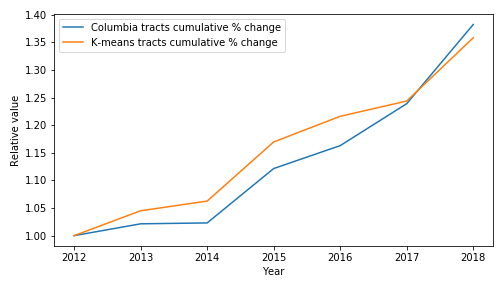
\includegraphics{figs/comparing_rv_in_g_tracts.png}}
    \caption{Comparing cumulative relative change in condominium values}
    \label{comparing_cum_perc_change_value}
\end{figure}

We plot the excess relative change for gentrified tracts identified by each method in Figure \ref{excess_rchange}. We see that the gentrified tracts identified by the Columbia method see very little excess increase over  
non-gentrified tracts up until 2016, after which a sharp increase in excess relative change occurs. The excess change for gentrified tracts identified by K-means, on the other hand, shows a far more gradual but consistent positive excess over non-gentrified tracts. But we are now faced with the question, how does this compare to the state of the general housing market in Manhattan? Specifically, how has the market driven this trend?

\begin{figure}[h]
    \centering
    \scalebox{0.5}  
    {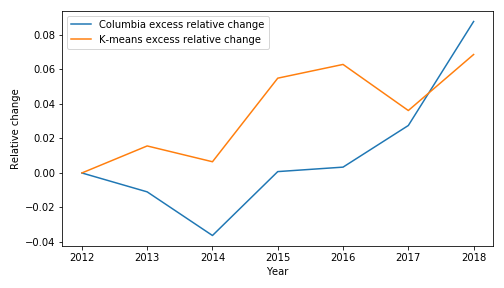
\includegraphics{figs/excess_rchange.png}}
    \caption{Excess relative change in condo prices}
    \label{excess_rchange}
\end{figure}

\subsection{The property market in Manhattan}

We are interested in the broad state of the housing market in New York City and more specifically, Manhattan. The magazine, \textit{New York Curbed}, has performed an analysis of the general property marked in the five boroughs of New York City \cite{Curbed analysis} and openly provides the datasets they used with total property sales per quarter from Q1 2010 to Q3 2019 and mean sale price for Manhattan for the same time frame. Analysing the state of the property market in Manhattan allows us to assess and explain excess relative change observed in the Section \ref{finding excess relative change}. 

Using the aforementioned datasets, we plot the number of sales per quarter for all boroughs in Figure \ref{sales_quarter_borough} where we see Manhattan dominating with most sales in the early half of the 2010's, ceding this title to Queens post approximately 2015. Plotting the relative change in sales for the period we are interested in, 2012-2018, (Figure \ref{manhattan_relative_sales}) we see that sales peak in 2013 and 2014 before generally declining. However, during this period the average sale price of properties in Manhattan has increased monotonically (Figure \ref{manhattan_mean_sale_price}) despite a reduction in overall sales leading to an overall increase in annual market value in Figure \ref{manhattan_market_size}, except for 2018. 

\begin{figure}[H]
    \centering
    \scalebox{0.5}  
    {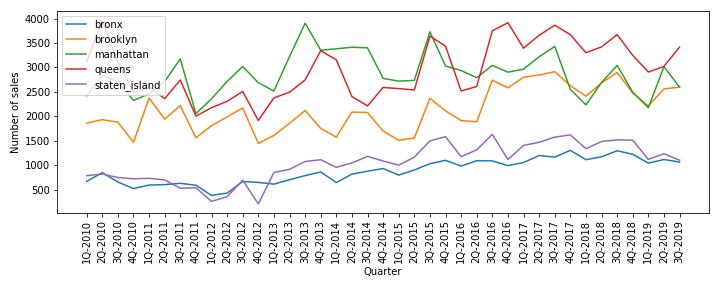
\includegraphics{figs/sales_by_borough_per_quarter.png}}
    \caption{Total sales per quarter}
    \label{sales_quarter_borough}
\end{figure}

\begin{figure}[H]
    \centering
    \scalebox{0.5}  
    {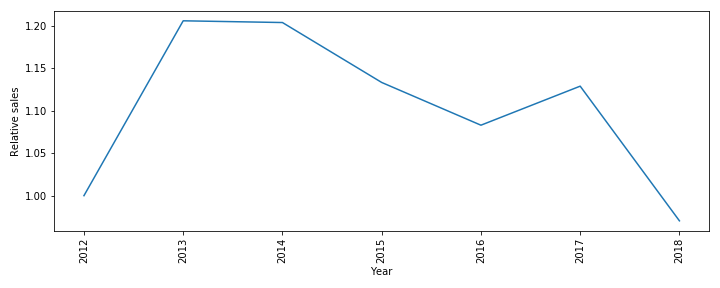
\includegraphics{figs/manhattan_relative_sales.png}}
    \caption{Manhattan relative property sales 2012-2018}
    \label{manhattan_relative_sales}
\end{figure}

\begin{figure}[H]
    \centering
    \scalebox{0.5}  
    {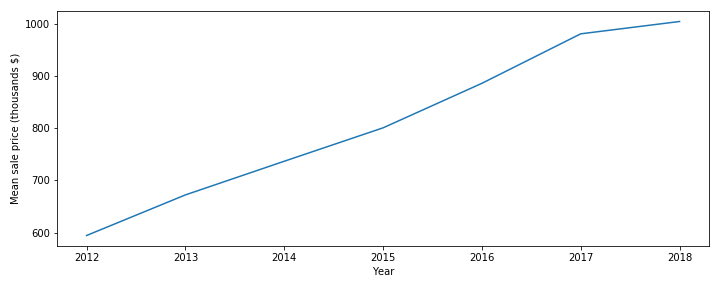
\includegraphics{figs/manhattan_mean_sale_price.png}}
    \caption{Manhattan mean sale price 2012-2018}
    \label{manhattan_mean_sale_price}
\end{figure}

\begin{figure}[H]
    \centering
    \scalebox{0.5}  
    {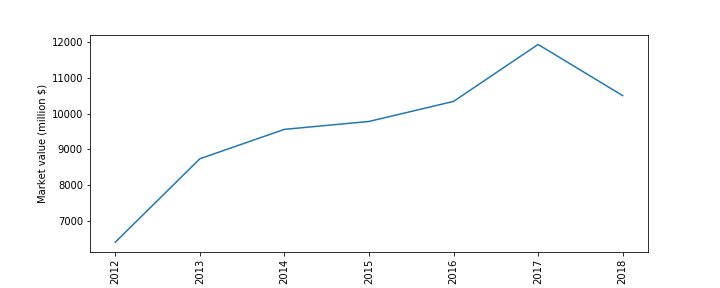
\includegraphics{figs/manhattan_property_market.png}}
    \caption{Manhattan property market value 2012-2018}
    \label{manhattan_market_size}
\end{figure}

2018 saw the worst performing Manhattan real estate market since 2009 as over the past decade \cite{CNBC Manhattan real estate}, lack of available land for new construction led to increasing land values which in turn encouraged any new properties to be built for the luxury market resulting in a lack of more affordable housing. Financial market performance in 2018 saw a souring of interest for Manhattan real estate from foreign investors leading to a declining property market. 

Figure \ref{columbia_summary} shows that condo price growth in areas identified as gentrified according to the Columbia methodology has occurred almost exclusively after 2016, merely two years after the decline in Manhattan's property sales began. This suggests that gentrification in Manhattan is a very recent phenomenon that has occurred in response to dwindling interest in the high value properties. In comparison, condominium prices in areas identified as gentrified by our K-means model (Figure \ref{k_means_summary}) identifies more tracts that have seen excess increase in condo prices far earlier with weak signs of excess increase prior to 2014 and far more significant excess increase after 2014, which corresponds to gentrification as a response to a reduction in property sales. With our K-means method, we are able to identify tracts undergoing gentrification earlier than with the Columbia method, as well as relate gentrification more closely to the state of the property market in the area. 

\begin{figure}[h]
\centering
\begin{subfigure}{.5\textwidth}
  \centering
  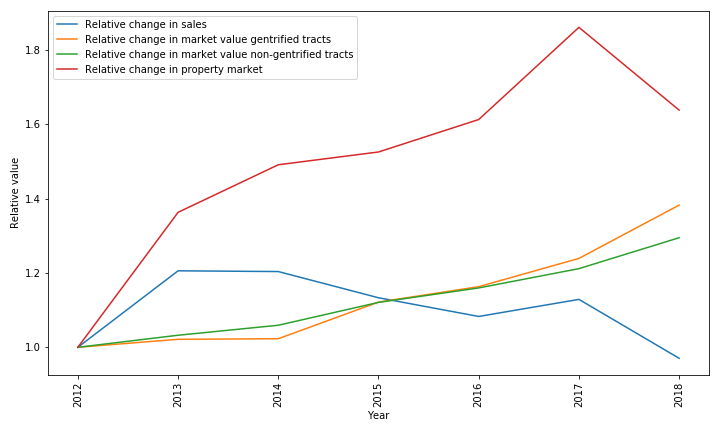
\includegraphics[width=1.0\linewidth]{figs/columbia_summary.png}
  \caption{Columbia method comparative plot}
  \label{columbia_summary}
\end{subfigure}%
\begin{subfigure}{.5\textwidth}
  \centering
  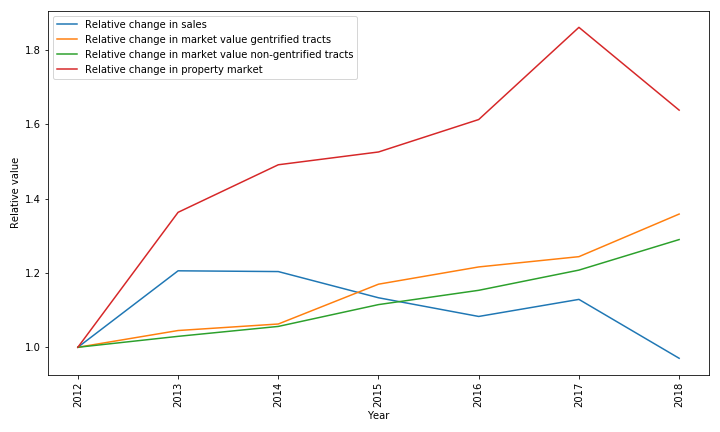
\includegraphics[width=1.0\linewidth]{figs/k_means_summary.png}
  \caption{K-means method comparative plot}
  \label{k_means_summary}
\end{subfigure}
\caption{Comparative plots for Columbia and K-means method results}
\label{methods_summary_plot}
\end{figure}

\subsection{Considering rental properties}

Thus far we have considered only the price of properties -- price is a direct indicator of the desirability and demand for housing in an area -- but we have failed to consider displacement. Renters are another key demographic in an area as they are ones that are likely to be 'priced out' of their homes during the process of gentrification. Yet we disregard this information with good reason; New York only provides data on evictions from the year 2017 \cite{Evictions data}. This limits the extent to which we can use evictions data to identify gentrified tracts, but in this study it provides a crucial way of evaluating the methodologies that find such tracts. 

We consider residential evictions in Manhattan that were completed in 2017 and 2018, although we note that eviction proceedings take on average twelve weeks in New York, in addition to up to six months a judge can award a tenant to stay in a property before eviction.

To enable comparison between evictions in gentrified and non-gentrified areas, we normalise total evictions by the number of GEOID tracts they occurred in thereby obtaining an average evictions per tract metric for 2017 and 2018. 

Figure \ref{columbia_evictions} shows that gentrified tracts identified by the Columbia method show significantly higher eviction rates than non-gentrified tracts with the eviction rate increasing in 2018 for these gentrified tracts. By contrast, in Figure \ref{k_means_evictions}, the K-means method gentrified tracts show a very similar eviction rate with both non-gentrified areas as well as across the two years. This potentially suggests that the Columbia method is more adept at recognising displacement due to gentrification, although more data of evictions throughout the 2012-2018 period would confirm this. 

\begin{figure}[h]
\centering
\begin{subfigure}{.5\textwidth}
  \centering
  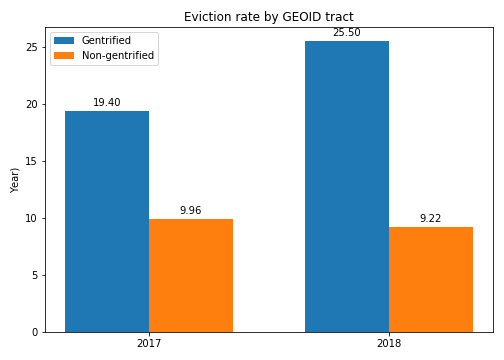
\includegraphics[width=1.0\linewidth]{figs/columbia_evictions.png}
  \caption{Columbia method}
  \label{columbia_evictions}
\end{subfigure}%
\begin{subfigure}{.5\textwidth}
  \centering
  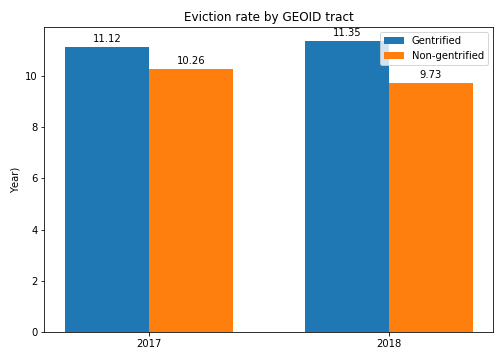
\includegraphics[width=1.0\linewidth]{figs/k_means_evictions.png}
  \caption{Our K-means method}
  \label{k_means_evictions}
\end{subfigure}
\caption{Evictions per tract for gentrified and non-gentrified tracts identified by Columbia and K-means methods}
\label{evictions}
\end{figure}


			
	\newpage
	
	\begin{thebibliography}{20} 
		
		\addcontentsline{toc}{section}{\refname}
		
		\bibitem{Chapple17} Chapple, Karen, et al. "Developing a new methodology for analyzing potential displacement." (2017).
		
		\bibitem{Freeman05} Freeman, Lance. "Displacement or succession? Residential mobility in gentrifying neighborhoods." \emph{Urban Affairs Review} 40.4 (2005): 463-491.
		
		\bibitem{Governing15} Maciag, Michael. “Gentrification Report Methodology” \emph{Governing} (2015) \url{https://www.governing.com/gov-data/gentrification-report-methodology.html}. Accessed 24 October 2020.
		
		\bibitem{Preis20} Preis, Benjamin, et al. "Mapping gentrification and displacement pressure: An exploration of four distinct methodologies." \emph{Urban Studies} (2020): 0042098020903011.
		
		\bibitem{Bhavsar20} Bhavsar, Kumar, Richman. "Defining gentrification for epidemiologic research: A systematic review." \emph{PLOS ONE}. 15(5):e0233361.
		
		\bibitem{BuzzFeed} Vo, Lam Thuy. "They Played Dominoes Outside Their Apartment For Decades. Then The White People Moved In And Police Started Showing Up" \emph{BuzzFeedNews} \url{https://www.buzzfeednews.com/article/lamvo/gentrification-complaints-311-new-york} Accessed 24 October 2020.
		
		\bibitem{DOF Condo Valuation dataset} 
        NYC Open Data DOF Condominium Comparable Rental Income in NYC.
        \url{https://data.cityofnewyork.us/City-Government/DOF-Condominium-Comparable-Rental-Income-in-NYC/9ck6-2jew}. Accessed 20 October 2020.
        
        \bibitem{BBL info}
        Borough, Block, Lot parcel number system. \url{https://en.wikipedia.org/wiki/Borough,_Block_and_Lot}. Accessed 20 October 2020.
        
        \bibitem{BBL to GEOID conversion} Finding the GEOID of an address. \url{https://geocoding.geo.census.gov/geocoder/geographies/onelineaddress?form}. Accessed 21 October 2020.
        
        \bibitem{Curbed analysis} NYC home prices nearly doubled in the 2010s. What do the 2020s hold? \url{https://ny.curbed.com/2019/12/13/21009872/nyc-home-value-2010s-manhattan-apartments}. Accessed 22 October 2020.
        
        \bibitem{CNBC Manhattan real estate} Manhattan real estate closes 2018 as worst year since the financial crisis. \url{https://www.cnbc.com/2019/01/02/manhattan-real-estate-closes-2018-as-worst-year-since-financial-crisis.html}. Accessed 23 October 2020.
        
        \bibitem{Evictions data} NYC Open Data Evictions \url{https://data.cityofnewyork.us/City-Government/Evictions/6z8x-wfk4}. Accessed 22 October 2020.
		
	\end{thebibliography}
	
\end{document}